\documentclass{beamer}
\usepackage{beamerthemeshadow}
\usetheme{Warsaw}
\usepackage{graphicx}
\usepackage{caption,subcaption}
%\usepackage[showframe]{geometry}
\usepackage{color}
\usepackage[utf8]{inputenc}
\usepackage{hyperref}
\usepackage[flushleft]{threeparttable}
\usepackage[T2A]{fontenc}
\usepackage[english,serbian]{babel}
\definecolor{beamer@darkerblue}{rgb}{0.1.5,0.2,0.35}
\definecolor{beamer@ibmblue}{rgb}{0.3,0.42,0.7}
\setbeamercolor{structure}{fg=beamer@ibmblue}
\setbeamercolor{section in head/foot}{bg=beamer@darkerblue}

\def\d{{\fontencoding{T1}\selectfont\dj}}
\def\D{{\fontencoding{T1}\selectfont\DJ}}

\title[]{Kompanija IBM}
\subtitle{-- Seminarski rad --}
\author[]{Staša Đorđević\and
Jovana Medenica\\\and  
Marko Veljović\and
Matija Radulović}
\institute[]{Matematički fakultet\\Univerzitet u Beogradu}
\date{
    \footnotesize{Beograd, 2022.}	
}

\begin{document}

\begin{frame}
	\thispagestyle{empty}
	\titlepage
\end{frame}

\begin{frame}[fragile]\frametitle{Literatura}
	\begin{itemize}
		\item Zasnovano na:\\
		...
		(\url{http://../})
	\end{itemize}
\end{frame}

\begin{frame}
	\frametitle{Pregled} % Table of contents slide, comment this block out to remove it
	\tableofcontents[hidesubsections] 
\end{frame}

\section{Rana istorija kompanije}

\begin{frame}[fragile]\frametitle{Nastanak kompanije IBM}
	\begin{itemize}	
		\item Koreni se naziru krajem 19. veka
		\item Postojale su četiri male kompanije koje su se kasnije spojile u IBM
		\item Herman Holerit - popis stanovništva 1890.
		\item Kompanija CTR kao preteča IBM-a
		\item Tomas J. Votson - THINK
		\item Od 1924. godine zvaničan naziv je IBM (eng.~{\em International Business Machines})
		\end{itemize}
\end{frame}

\section{IBM sredinom proslog veka}

\begin{frame}[fragile]\frametitle{IBM sredinom proslog veka}
	\begin{itemize}	
		\item Uticaj Velike ekonomske krize na kompaniju
		\item Ugovor sa američkom vladom - ključan potez za prolazak kroz težak period
		\item Beneficije za zaposlene za vreme krize
            \item Drugi svetski rat, stanje kompanije za vreme sukoba svetskih razmera
            \item Privremeno prilagođavanje proizvodnje novom tržištu
            \item Smrt Votsona Seniora, dolazak mlađe generacije
            \item Zlatno doba
	\end{itemize}
\end{frame}



\begin{frame}[fragile]\frametitle{Najbitniji izumi}
	\begin{itemize}	
		\item IBM 603, 701
		\item IBM 650, 1401	
		\item Porodica računara Sistem/360
		\item IBM 5100, PC
		\item Magnetna traka, hard disk, flopi disk, DRAM
		\item Relacione baze, SQL
		\item Nobelove nagrade, standardi i protokoli, STM, RISC, UPC, itd.
		\end{itemize}
\end{frame}
\begin{frame}[fragile]\frametitle{Najbitniji izumi}
	\begin{figure}[htb]\captionsetup[subfigure]{labelformat=empty}
    \centering 
\begin{subfigure}{0.25\textwidth}
  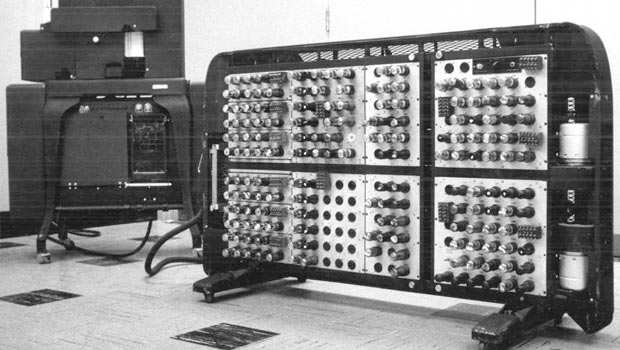
\includegraphics[width=\linewidth]{ibm603.jpg}
  \caption{IBM 603}
  \label{fig:1}
\end{subfigure}\hfil
\begin{subfigure}{0.25\textwidth}
  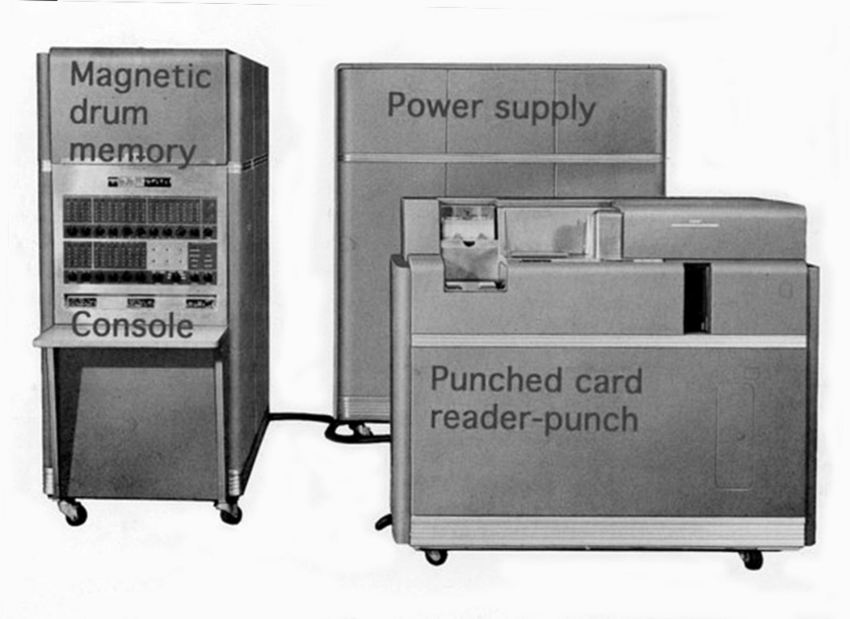
\includegraphics[width=\linewidth]{ibm650.png}
  \caption{IBM 650}
  \label{fig:2}
\end{subfigure}\hfil
\begin{subfigure}{0.25\textwidth}
  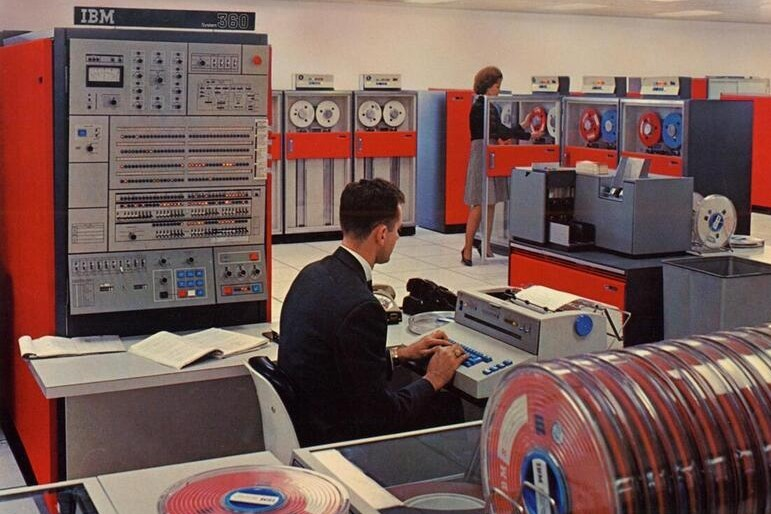
\includegraphics[width=\linewidth]{sys360.jpg}
  \caption{Sistem 360}
  \label{fig:3}
\end{subfigure}

\medskip
\begin{subfigure}{0.25\textwidth}
  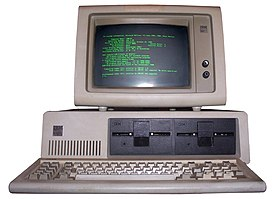
\includegraphics[width=\linewidth]{ibmpc.jpg}
  \caption{IBM PC}
  \label{fig:4}
\end{subfigure}\hfil 
\begin{subfigure}{0.25\textwidth}
  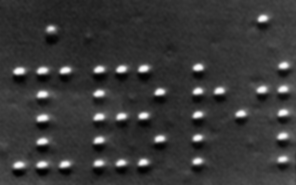
\includegraphics[width=\linewidth]{ibm_atom.png}
  \caption{IBM ispisan atomima}
  \label{fig:5}
\end{subfigure}\hfil 
\begin{subfigure}{0.25\textwidth}
  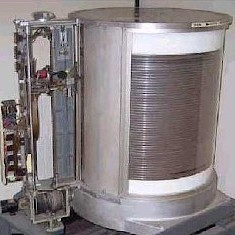
\includegraphics[width=\linewidth]{ramac_hdd.jpg}
  \caption{Prvi hard disk}
  \label{fig:6}
\end{subfigure}
\label{fig:images}
\end{figure}
\end{frame}
\section{Razvoj ličnih računara i pad IBM-a}
\begin{frame}[fragile]\frametitle{Razvoj ličnih računara i pad IBM-a}
	\begin{itemize}
	\item Propust u razvoju minikompjutera, nije ispratila tržište
	\item Povratak u doba ličnih računara
	\begin{itemize}
	\item IBM 5100
	\item IBM PC
	\item IBM PC AT
	\end{itemize}
	\item Pravi niz pogrešnih odluka koje je skupo koštaju
	\item Proizvodnju operativnog sistema prepušta Majkrosoftu(eng.~{\em Microsoft})
	\item Proizvodnju mikroprocesora prepušta Intelu
	\item Da bi se povratila menja fokus sa hardvera na razvoj softvera
	\end{itemize}
\end{frame}



\section{IBM danas}

\begin{frame}[fragile]\frametitle{IBM danas}
	\begin{itemize}	
		\item ...
		\item ...
		\item ...
	\end{itemize}
\end{frame}

\section{Zakljucak}

\begin{frame}[fragile]\frametitle{Zakljucak}
	\begin{itemize}	
		\item ...
		\item ...
	\end{itemize}
\end{frame}


\end{document}